\documentclass[letterpaper]{article}
\topmargin=0.8cm
\oddsidemargin=-0.25in
\voffset=-0.9in
\textwidth=7in
\textheight=9.25in
\headsep=36pt
\headheight=24pt
\linespread{1.1}
\usepackage{amsmath,amssymb,amsfonts,mathtools,bm}
\usepackage{booktabs,array,graphicx,float}
\usepackage{microtype,xcolor}
\usepackage{tikz,pgfplots}\pgfplotsset{compat=1.18}
\usepackage[algoruled,linesnumbered,vlined,titlenotnumbered]{algorithm2e}
\usepackage[linkcolor=black,colorlinks=true,urlcolor=blue,citecolor=black]{hyperref}
\usepackage{fancyhdr,lastpage}
\usepackage[yyyymmdd,hhmmss]{datetime}
\definecolor{revisionblue}{RGB}{0,74,173}
\newcommand{\E}{\mathbb E}
\newcommand{\Var}{\operatorname{Var}}
\newcommand{\Cov}{\operatorname{Cov}}
\newcommand{\Normal}{\mathcal N}
\newcommand{\calD}{\mathcal D}
\newcommand{\diag}{\operatorname{diag}}
\newcommand{\Remax}{\operatorname{Remax}}
\newcommand{\ind}{\mathbb 1}
\newcommand{\dd}{\,\mathrm d}
\newcommand{\vbar}{\overline{V^2}}
\newcommand{\vbari}{\overline{V_i^2}}
\newcommand{\given}{\mid}
\newcommand{\courseS}{TAGI-V--Remax Calibration}
\newcommand{\deptS}{Polytechnique Montréal}
\newcommand{\profS}{J.A. Goulet, L.H. Nguyen \& M. Florensa-Montilla}
\newcommand{\dateS}{\today}
\newcommand{\titleS}{~}
\pagestyle{fancy}
\fancyhead{}
\fancyhead[c]{\scshape\courseS\hfill\normalfont\profS\\\raggedright\deptS\hfill\dateS}
\fancyfoot{}
\fancyfoot[l]{\tiny (Last update : \today, \currenttime)\\[6pt]}
\fancyfoot[c]{\thepage/\pageref{LastPage}}
\hypersetup{pdftitle={CDF TAGI-V and Auxiliary Gaussian Calibration with Remax},pdfauthor={J.-A. Goulet, L.-H. Nguyen, and M. Florensa-Montilla}}
\begin{document}
\title{\titleS}
\section{Context}\label{S:scope}
This note follows the original \emph{Hierarchical Softmax Calibration} formulation supplied as \nolinkurl{HSM_calibration_Goulet_Nguyen_Florensa.original.tex}. Its central design separates two inference channels: the network learns in logit space, while an auxiliary Gaussian observation model uses out-of-sample class labels to learn calibration parameters only. Here that design is extended to a TAGI-V network and a multiclass Remax output.

The construction has three parts.
\begin{enumerate}
\item Retain TAGI-V's prediction and variance heads, with Gaussian latent outputs $(\bm Z^{(\mathtt O)},\bm U)$. Replace the exponential variance activation by $\vbari=\varepsilon+\kappa\Phi(U_i)$, where $\varepsilon,\kappa>0$. Train the network or just its final Bayesian layer using Gaussian logit observations (\S\ref{S:gaussian}).
\item Propagate the prediction uncertainty and $V_i\given U_i\sim\Normal(0,\vbari)$ through Remax. Both the MM-Remax approximation and the more accurate Laplace-transform integration are specified (\S\ref{S:laplace}, \S\ref{S:mm}).
\item Learn a shared Gaussian calibration state through a separate, sequential probability observation channel (\S\ref{S:calibration}). This channel uses forward predictions and updates only the calibration state, as in the intended source.
\end{enumerate}
The key adaptation is where calibration acts. Since $\Remax(g\bm x)=\Remax(\bm x)$ for any $g>0$, an ordinary global logit gain disappears. Instead define a positive deviation scale $s=e^L$, with Gaussian state $L$, and use
\begin{equation}
\boxed{\bm X_L=\bm\mu+e^L[(\bm Z^{(\mathtt O)}-\bm\mu)+\bm V],\qquad
\bm p=\E[\Remax(\bm X_L)].}
\label{E:contextmodel}
\end{equation}
This rescales combined epistemic and aleatoric deviations while retaining the predictive logit mean $\bm\mu$. The original Gaussian-gain \emph{observation-update design} is retained, while its gain location and positivity parameterization are adapted to Remax. A Gaussian $L$ replaces the original unrestricted Gaussian $G$ so that $s>0$ for every realization; clipping a Gaussian gain mean would not ensure positive draws.

Notation follows the pasted TAGI/TAGI-V formulation: $Z_i$ abbreviates $Z_i^{(\mathtt O)}$, $C\in\{1,\ldots,K\}$ is the observed class, and $\bm A$ denotes Remax probabilities, distinct from hidden activations $\bm A^{(j)}$. The standard normal density and CDF are $\varphi$ and $\Phi$. Exact identities below are distinguished from Gaussian projections and numerical approximations. Direct categorical training, which changes the training likelihood, is retained only as an optional extension in Appendix~\ref{S:training}.

\section{TAGI backbone and a CDF variance head}\label{S:cdf}
\subsection{Gaussian propagation and the two outputs}
For a fully connected layer, retain
\begin{equation}
Z_i^{(j+1)}=\sum_k W_{i,k}^{(j)}A_k^{(j)}+B_i^{(j)}.
\end{equation}
TAGI propagates moments using GMA and appropriate activation moment rules, and projects states back to Gaussian distributions. For jointly Gaussian $X_1,X_2,X_3$, with $c_{ab}=\Cov(X_a,X_b)$, the GMA identities used here are
\begin{align}
\E[X_1X_2]&=\mu_1\mu_2+c_{12},\\
\Var(X_1X_2)&=\sigma_1^2\sigma_2^2+c_{12}^2+2c_{12}\mu_1\mu_2+\sigma_1^2\mu_2^2+\sigma_2^2\mu_1^2,\\
\Cov(X_3,X_1X_2)&=c_{13}\mu_2+c_{23}\mu_1.
\end{align}
The product distribution itself need not be Gaussian. The same distinction applies to transformed variance states: moment matching is not a support-preserving Gaussian distributional identity.

The last hidden layer feeds two sets of weights:
\begin{equation}
Z_i=\sum_k W^{(\mathtt L)}_{Z,i,k}A_k^{(\mathtt L)}+B^{(\mathtt L)}_{Z,i},\qquad
U_i=\sum_k W^{(\mathtt L)}_{U,i,k}A_k^{(\mathtt L)}+B^{(\mathtt L)}_{U,i}.
\end{equation}
The working TAGI approximation at an input $\bm x$ is
\begin{equation}
q(\bm z,\bm u\given\bm x)=\prod_{i=1}^K
\Normal(z_i;\mu_i,e_i)\Normal(u_i;\nu_i,r_i),
\quad e_i=\sigma_{Z_i}^2,\quad r_i=\sigma_{U_i}^2.
\label{E:factorization}
\end{equation}
This explicitly discards cross-class and cross-head correlations at the output. Shared features generally create such correlations in the full model. Exactness statements below are conditional on this approximation, not claims about the exact network posterior. Appendix~\ref{A:correlated} describes the extension to a correlated $(Z_i,U_i)$ pair.

\subsection{Positive, bounded aleatoric variance}
Define
\begin{equation}
\boxed{\vbari=h(U_i):=\varepsilon+\kappa\Phi(U_i),\qquad \varepsilon>0,\quad\kappa>0.}
\label{E:head}
\end{equation}
For every finite $U_i$, $\varepsilon<\vbari<\varepsilon+\kappa$. Thus a CDF activation provides an upper bound as well as positivity. The constants have units of squared logits and should be fixed before calibration. If a different cap or a standardized argument $(U_i-b)/a$ is desired, it is a model choice to be stated and selected on training/validation data. The cap should accommodate the intended logit scale; a saturating head can cease to adapt.

Let
\begin{equation}
a_i=\frac{\nu_i}{\sqrt{1+r_i}},\qquad \rho_i=\frac{r_i}{1+r_i},
\end{equation}
and let $\Phi_2(\cdot,\cdot;\rho)$ denote the bivariate standard normal CDF. The following moments are exact for the Gaussian $U_i$ in \eqref{E:factorization}:
\begin{align}
h_i:=\E[\vbari]&=\varepsilon+\kappa\Phi(a_i),\label{E:hmean}\\
b_i:=\Var(\vbari)&=\kappa^2\left[\Phi_2(a_i,a_i;\rho_i)-\Phi(a_i)^2\right],\label{E:hvar}\\
c_{U_i,h}:=\Cov(U_i,\vbari)&=\frac{\kappa r_i}{\sqrt{1+r_i}}\varphi(a_i).\label{E:hc}
\end{align}
More generally, for any state $T$ jointly Gaussian with $U_i$,
\begin{equation}
\Cov(T,\vbari)=\frac{\kappa\Cov(T,U_i)}{\sqrt{1+r_i}}\varphi(a_i).
\label{E:upstreamcdf}
\end{equation}
These identities follow from normal probability augmentation and Stein's identity. They supply the CDF forward moments and the cross-covariance needed for an RTS interface. If a legacy variance module supplies posterior moments $(h_i^+,b_i^+)$, its Gaussian bridge to $U_i$ is
\begin{equation}
\nu_i^+=\nu_i+\frac{c_{U_i,h}}{b_i}(h_i^+-h_i),\qquad
r_i^+=r_i+\left(\frac{c_{U_i,h}}{b_i}\right)^2(b_i^+-b_i).
\label{E:cdfbridge}
\end{equation}
This last bridge is a Gaussian projection, not an exact inverse of the CDF; it is omitted when the likelihood updates $U_i$ directly. For $b_i=0$, use the degenerate-state limit instead of dividing by zero. Future positive variances are always generated from $h(U_i)$, not sampled from a Gaussian approximation to $\vbari$.

\subsection{A random variance is different from a Gaussian error}
Introduce independent standard normal innovations $\xi_i$ and set
\begin{equation}
V_i=\sqrt{h(U_i)}\,\xi_i,\qquad
V_i\given U_i\sim\Normal(0,h(U_i)).
\label{E:noise}
\end{equation}
Conditionally, the error is Gaussian. Marginally it is a Gaussian variance mixture. In particular,
\begin{align}
\E[V_i]&=0,& \Var(V_i)&=h_i,& \Cov(Z_i,V_i)&=0,\label{E:noise2}\\
\E[V_i^4]&=3(h_i^2+b_i),&\Var(V_i^2)&=2h_i^2+3b_i,&\Cov(\vbari,V_i^2)&=b_i.
\label{E:noise4}
\end{align}
Consequently, $b_i$ is uncertainty \emph{about} a variance; it is not another variance to add to $e_i+h_i$. It enters fourth moments and nonlinear predictive averages. Substituting $2h_i^2$ for $\Var(V_i^2)$ discards variance-head uncertainty. Also $\Cov(U_i,V_i)=0$, even though $U_i$ controls the distribution of $V_i$; a purely linear Gaussian update on the raw residual cannot by itself identify this head. This motivates AGVI's squared-error channel or the likelihood tilts developed below.

\section{Where a joint calibration scale can act}\label{S:scale}
\subsection{Why ordinary temperature scaling disappears}
Fix the all-zero convention
\begin{equation}
\Remax_i(\bm x)=
\begin{cases}
[x_i]_+/\sum_j[x_j]_+,&\sum_j[x_j]_+>0,\\
1/K,&\sum_j[x_j]_+=0,
\end{cases}
\qquad [x]_+=\max(0,x).
\label{E:remax}
\end{equation}
For any $g>0$, the positive homogeneity of ReLU gives
\begin{equation}
\boxed{\Remax(g\bm x)=\Remax(\bm x).}\label{E:invariance}
\end{equation}
The all-zero event is unchanged by $g$, so the identity also holds there. It remains true for a random positive $g$, regardless of dependence on $\bm x$. Thus $\Remax(e^L(\bm Z+\bm V))$ cannot learn a useful global gain. A numerical implementation that changes under this operation is changing an approximation, not the target Remax distribution.

\subsection{Scale deviations while fixing the predictive mean}
After training, freeze $q$ and its input-dependent mean $\bm\mu$. Introduce a single shared log-scale $L$, initially $L\sim\Normal(\lambda_0,q_0)$, and define
\begin{equation}
\boxed{
X_{i,l}=\mu_i+s(l)(Z_i-\mu_i+V_i),\qquad s(l)=e^l.
}\label{E:calibratedlogit}
\end{equation}
The scalar is a \emph{standard-deviation} multiplier. Equivalently, by \eqref{E:invariance},
\begin{equation}
\Remax(\bm X_l)=\Remax\!\left(e^{-l}\bm\mu+(\bm Z-\bm\mu)+\bm V\right).
\label{E:equivmean}
\end{equation}
This equivalent form makes explicit that the learnable quantity is the mean relative to uncertainty. Both epistemic deviations and aleatoric noise receive the same scale:
\begin{equation}
\E[X_{i,l}]=\mu_i,\quad
v_{i,\mathrm{epi}}(l)=e^{2l}e_i,\quad
v_{i,\mathrm{ale}}(l)=e^{2l}h_i,\quad
\Var(X_{i,l})=e^{2l}(e_i+h_i).
\label{E:totalvariance}
\end{equation}
The epistemic-to-aleatoric ratio is retained in logit space. The operation is a calibrated predictive distribution around a frozen posterior mean, not a claim to have recomputed the Bayesian weight posterior. If $L\sim\Normal(\lambda,q)$ is subsequently used, $\Var(X_{i,L})=e^{2\lambda+2q}(e_i+h_i)$; integrating this variance into a single Gaussian is an additional approximation.

Conditional on $U_i=u$ and $L=l$, the working model is particularly simple:
\begin{equation}
X_{i,l}\given u\sim\Normal\!\left(\mu_i,e^{2l}[e_i+h(u)]\right).
\label{E:conditionalx}
\end{equation}
Given $l$, distinct $X_{i,l}$ remain independent after integrating their separate $U_i$. Integrating a \emph{shared} $L$ creates dependence, even when off-diagonal logit covariances are zero. Therefore the class products used below must be computed conditionally on $l$ before averaging over it.

\paragraph{Identifiability and limits.}
A global $L$ does not separately correct the epistemic and aleatoric magnitudes. Separate scales $e^{L_E}(Z_i-\mu_i)$ and $e^{L_A}V_i$ are possible, but can be weakly identified by labels and require more calibration data. Fix the variance cap and network while learning the default scalar. If all $\mu_i=0$, \eqref{E:calibratedlogit} reduces to the invariant case and $L$ is completely unidentified. If the classes are exchangeable, marginal probabilities can also remain uniform for all $l$. As $s\to\infty$, probabilities need not tend to $1/K$ when class variances differ. Increasing $s$ need not monotonically increase entropy or preserve the predicted class.

\section{Laplace-Remax with a random CDF variance head}\label{S:laplace}
\subsection{Per-class kernels}
For a Gaussian $X\sim\Normal(m,d^2)$, $d>0$, write
\begin{equation}
\alpha=m/d,\qquad \beta(t)=\alpha-dt,\qquad c(t)=\exp(-mt+d^2t^2/2).
\end{equation}
For $M=[X]_+$, define
\begin{align}
\mathcal L(t;m,d)&:=\E[e^{-tM}]=\Phi(-\alpha)+c(t)\Phi(\beta),\\
\mathcal D(t;m,d)&:=\E[Me^{-tM}]=c(t)[(m-d^2t)\Phi(\beta)+d\varphi(\beta)],\\
\mathcal F(t;m,d)&:=\E[M^2e^{-tM}]\nonumber\\
&=c(t)\left[\{(m-d^2t)^2+d^2\}\Phi(\beta)+(m-d^2t)d\varphi(\beta)\right].
\label{E:kernels}
\end{align}
These are the Gaussian kernels in the supplied Laplace-Remax note. To retain uncertainty in $\vbari$, average each kernel \emph{before} taking products across classes. For $d_i(u,l)=e^l\sqrt{e_i+h(u)}$, set
\begin{align}
L_i(t\given l)&=\E_{U_i}[\mathcal L(t;\mu_i,d_i(U_i,l))],\\
D_i(t\given l)&=\E_{U_i}[\mathcal D(t;\mu_i,d_i(U_i,l))],\\
F_i(t\given l)&=\E_{U_i}[\mathcal F(t;\mu_i,d_i(U_i,l))],\\
\pi_{0,i}(l)&=\E_{U_i}\left[\Phi\!\left(-\mu_i/d_i(U_i,l)\right)\right].
\label{E:mixturekernels}
\end{align}
All expectations in \eqref{E:mixturekernels} are scalar Gaussian integrals. Define
\begin{equation}
P(t\given l)=\prod_jL_j(t\given l),\qquad \pi_0(l)=\prod_j\pi_{0,j}(l).
\end{equation}
The $K$-dimensional integration over the independent variance heads therefore reduces to $K$ separate one-dimensional integrations. This is more faithful than replacing each head by $h_i$ and then treating the combined logit as exactly Gaussian.

\subsection{Probability moments}
Let $A_{i,l}=\Remax_i(\bm X_l)$, $m_i(l)=\E[A_{i,l}]$, and $B_{ij}(l)=\E[A_{i,l}A_{j,l}]$. Using $1/S=\int_0^\infty e^{-tS}\dd t$ and $1/S^2=\int_0^\infty t e^{-tS}\dd t$ for $S>0$ gives
\begin{align}
\boxed{m_i(l)=\int_0^\infty D_i(t\given l)\frac{P(t\given l)}{L_i(t\given l)}\dd t+\frac{\pi_0(l)}K,}\label{E:pmean}\\
B_{ii}(l)&=\int_0^\infty tF_i(t\given l)\frac{P(t\given l)}{L_i(t\given l)}\dd t+\frac{\pi_0(l)}{K^2},\label{E:psecond}\\
B_{ij}(l)&=\int_0^\infty tD_i(t\given l)D_j(t\given l)
\frac{P(t\given l)}{L_i(t\given l)L_j(t\given l)}\dd t+\frac{\pi_0(l)}{K^2},\quad i\ne j.
\label{E:pcross}
\end{align}
These are exact integral identities under \eqref{E:factorization} and the hierarchical noise model. Finite quadrature introduces numerical error. Ratios of products are mathematical shorthand; evaluate products excluding the selected indices or stable log-products in code.

For a fitted scale distribution $q_{\rm cal}(l)$, the final output moments are
\begin{equation}
\bm p=\E_L[\bm m(L)],\qquad
\bm\Sigma_{\bm A}=\E_L[\bm B(L)]-\bm p\bm p^\intercal.
\label{E:finalmoments}
\end{equation}
The exact moments satisfy
\begin{equation}
\sum_ip_i=1,\qquad \bm\Sigma_{\bm A}\bm 1=\bm 0,\qquad
\bm\Sigma_{\bm A}\succeq0,\qquad 0\le(\bm\Sigma_{\bm A})_{ii}\le p_i(1-p_i).
\label{E:simplexchecks}
\end{equation}
The all-zero correction is required even though $\E[[X_i]_+]>0$. A positive expectation does not eliminate the point mass at zero. With the positive noise floor, finite means, and finite $l$, the Gaussian conditional model assigns positive probability to the relevant sign events.

\paragraph{Cost.}
With $Q$ Laplace nodes, $J$ variance-head nodes, and $H$ scale nodes, means and diagonal second moments cost $O(HQJK)$. Full probability cross-moments add $O(HQK^2)$. This is not a finite closed-form formula: it is deterministic low-dimensional quadrature. Linear scaling in $K$ assumes fixed quadrature orders; the orders must be checked as the parameter range changes.

\section{Gaussian-channel TAGI-V with the CDF head}\label{S:gaussian}
The main training channel retains the observation model in the supplied TAGI-V description,
\begin{equation}
Y_i^{(Z)}=Z_i+V_i,\qquad V_i\given U_i\sim\Normal(0,h(U_i)).
\label{E:gausschannel}
\end{equation}
For classification, specify a fixed encoding; to retain the signed targets in the intended source, take $y_i^{(Z)}=2\ind_{c=i}-1\in\{-1,+1\}$ for all $K$ output units. A one-hot $0/1$ encoding is an alternative, but it changes the logit origin and therefore the Remax model. These are logit-space pseudo-observations, not measured probabilities. Their scale and offset affect Remax and must be fixed. The probabilistic model in this section is a surrogate for classification; its learned $h_i$ describes residual dispersion for that encoding.

The original AGVI strategy infers error moments and then updates $\vbari$ via $V_i^2$. With a bounded transform, a scalar variance-head quadrature can instead compute the posterior moments directly under the same Gaussian observation model. This avoids mixing a Gaussian marginal fourth moment with a random-variance hierarchy. Let $d_i(u)=e_i+h(u)$, $\Delta_i=y_i^{(Z)}-\mu_i$, and define
\begin{equation}
\omega_i(u)=\Normal(u;\nu_i,r_i)\Normal(y_i^{(Z)};\mu_i,d_i(u)),\qquad
\widetilde\omega_i(u)=\frac{\omega_i(u)}{\int\omega_i(t)\dd t}.
\label{E:gaussweights}
\end{equation}
The head update is
\begin{equation}
\nu_i^+=\int u\widetilde\omega_i(u)\dd u,\qquad
r_i^+=\int u^2\widetilde\omega_i(u)\dd u-(\nu_i^+)^2.
\label{E:ugauss}
\end{equation}
Conditionally on $u$ and the observation,
\begin{align}
\mu_{Z_i\given y,u}&=\mu_i+\frac{e_i}{d_i(u)}\Delta_i,&
v_{Z_i\given y,u}&=\frac{e_ih(u)}{d_i(u)},\\
\mu_{V_i\given y,u}&=\frac{h(u)}{d_i(u)}\Delta_i,&
v_{V_i\given y,u}&=\frac{e_ih(u)}{d_i(u)}.
\end{align}
The updated prediction-head moments follow by total expectation and variance:
\begin{equation}
\mu_{Z_i}^+=\E_{\widetilde\omega_i}[\mu_{Z_i\given y,U_i}],\quad
(\sigma_{Z_i}^2)^+=\E_{\widetilde\omega_i}[v_{Z_i\given y,U_i}+\mu_{Z_i\given y,U_i}^2]-(\mu_{Z_i}^+)^2.
\label{E:zgauss}
\end{equation}
The error and variance-head moments can likewise be obtained as
\begin{equation}
\E[V_i^2\given y]=\E_{\widetilde\omega_i}[v_{V_i\given y,U_i}+\mu_{V_i\given y,U_i}^2],\qquad
\E[\vbari\given y]=\E_{\widetilde\omega_i}[h(U_i)].
\end{equation}
These two expectations are not the same posterior quantity: observing a residual conveys information about its realized square and about its generating variance differently. Project $(Z_i,U_i)$ to the desired Gaussian structure and use \eqref{E:rts}. The formulas are exact scalar integral identities for the assumed independent Gaussian prior heads; this is a quadrature alternative to AGVI's two-stage Gaussian closure, not a claim that the published AGVI algorithm already uses these updates.

A minimal change to a legacy implementation is instead to keep its stated AGVI updates and replace only the exponential forward moments and activation cross-covariances with \eqref{E:hmean}--\eqref{E:upstreamcdf}. That route must retain the implementation's explicit Gaussian closure assumptions. In either case, use disjoint calibration labels for the auxiliary channel in \S\ref{S:calibration}; do not process a training label through both this Gaussian channel and an independent categorical channel.

\subsection{Return to the TAGI backward pass}
Collect the output heads in $\bm H=[\bm Z;\bm U]$. With their projected posterior moments available, use the supplied RTS structure. For any preceding state or parameter block $\bm T$ linked to $\bm H$,
\begin{align}
\mathbf J_{\bm T}&=\bm\Sigma_{\bm T\bm H}\bm\Sigma_{\bm H}^{-1},\\
\bm\mu_{\bm T}^+&=\bm\mu_{\bm T}+\mathbf J_{\bm T}(\bm\mu_{\bm H}^+-\bm\mu_{\bm H}),\\
\bm\Sigma_{\bm T}^+&=\bm\Sigma_{\bm T}+\mathbf J_{\bm T}(\bm\Sigma_{\bm H}^+-\bm\Sigma_{\bm H})\mathbf J_{\bm T}^\intercal.
\label{E:rts}
\end{align}
Use the corresponding next-layer state in subsequent recursive steps. The diagonal TAGI approximation projects the necessary covariance blocks accordingly. Because the two heads use the same observation, their posterior moments are inferred jointly through the Gaussian residual model, or through the single categorical tilt in Appendix~\ref{S:training}; they are not two independent copies of the label likelihood.

For an implementation using normalized additive state deltas, set
\begin{equation}
\delta\mu_{T_j}=\frac{\mu_{T_j}^+-\mu_{T_j}}{\sigma_{T_j}^2},\qquad
\delta S_{T_j}=\frac{(\sigma_{T_j}^2)^+-\sigma_{T_j}^2}{(\sigma_{T_j}^2)^2}.
\label{E:deltas}
\end{equation}
These are information-like deltas, not raw posterior moment differences. A regression coefficient $\Cov(A_i,Z_j)/\Var(Z_j)$ is an activation propagation coefficient, whereas the RTS gain that maps raw $\bm A$ posterior changes to $\bm Z$ uses $\bm\Sigma_{\bm Z\bm A}\bm\Sigma_{\bm A}^{-1}$. The conventions must not be interchanged. For zero prior variance the state is deterministic and its update uses the corresponding limit.

\section{Learning the shared scale through an auxiliary channel}\label{S:calibration}
\subsection{Which channel learns what}
The Gaussian training channel in \S\ref{S:gaussian} updates the network's prediction and variance heads and, through RTS, its trainable parameters. The auxiliary channel below updates only $L$. At each calibration sample, the network enters solely through the frozen forward summaries $(\bm\mu,\bm e,\bm\nu,\bm r)$. A validation/calibration pass can be run after an epoch, as in the intended source. Post-update training moments are not suitable calibration inputs, because they have already assimilated the label.

For a current calibration state $L\sim\Normal(\lambda,q)$, compute conditional Remax moments $m_i(l)=\E[A_i\given L=l]$ and $B_{ii}(l)=\E[A_i^2\given L=l]$ using \S\ref{S:laplace}. Then
\begin{align}
p_i&=\E_L[m_i(L)],&v_{A_i}&=\E_L[B_{ii}(L)]-p_i^2,\\
c_i:=\Cov(L,A_i)&=\E_L[(L-\lambda)m_i(L)]
=q\,\E_L[m_i'(L)].
\label{E:auxmoments}
\end{align}
The covariance expectation is evaluated directly by scalar quadrature; differentiating an approximate moment formula produces an approximate covariance, not an exact one. This is the counterpart of the gain/probability cross-covariance in the original note. A shared state is integrated once for the complete class probability, after the conditional class products have been formed.

\subsection{Observed-class Gaussian channel}
Fix the observed class $c$ and write $B_c=\ind_{C=c}$. The event $B_c=1$ has likelihood $A_c$ conditionally on the latent probability vector, so observing it gives the same exact likelihood as observing $C=c$. The Bernoulli total-variance identity gives
\begin{equation}
R_c:=\E[A_c(1-A_c)]=p_c(1-p_c)-v_{A_c},\qquad
\Var(B_c)=v_{A_c}+R_c=p_c(1-p_c).
\label{E:auxR}
\end{equation}
Thus the Gaussian surrogate $\widetilde Y_c=A_c+E_c$, with independent $E_c\sim\Normal(0,R_c)$, has the same unconditional mean, variance, and covariance with $L$. Its noise $E_c$ is a moment-matching device and is distinct from the TAGI-V logit error $V_i$. The latter has already been integrated into $A_c$ and must not be added again to \eqref{E:auxR}.

As in the intended source, construct only the two-variable joint surrogate
\begin{equation}
\begin{bmatrix}L\\\widetilde Y_c\end{bmatrix}\ \dot\sim\ \Normal\!\left(
\begin{bmatrix}\lambda\\p_c\end{bmatrix},
\begin{bmatrix}q&c_c\\c_c&p_c(1-p_c)\end{bmatrix}\right).
\end{equation}
Conditioning on the observed event $B_c=1$ yields the auxiliary update
\begin{equation}
\boxed{\lambda^+=\lambda+\frac{c_c}{p_c},\qquad
q^+_{\rm event}=q-\frac{c_c^2}{p_c(1-p_c)}.}
\label{E:auxupdate}
\end{equation}
Neither $\bm Z$ nor $\bm U$ is a variable of this auxiliary joint surrogate, so neither head receives a calibration update. Only $p_c$ and $c_c$ are needed for the recursion; the second moment is needed to interpret $R_c$ and report predictive uncertainty.

For exact moments under the current working prior, the mean step is exact for the categorical likelihood:
\begin{equation}
\E[L\given C=c]=\frac{\E[LA_c]}{p_c}=\lambda+\frac{c_c}{p_c}.
\end{equation}
The variance step is a Gaussian projection. It equals the exact posterior variance averaged over the binary partition $\{C=c,C\ne c\}$, not the variance conditional on the realized class. This distinction mirrors the original note. For $K>2$, there is no tree-node factorization to exploit: perform one observed-class event update per sample, and do not assimilate the other $K-1$ zero indicators as independent Bernoulli observations.

With exact moments, $c_c^2\le q\,p_c(1-p_c)$ follows from Cauchy--Schwarz applied to $(L,B_c)$. Approximate moments must be checked for consistency. If $q$ is small, $c_c\approx q\,m_c'(\lambda)$ and the mean step is approximately $q\,\partial_l\log m_c(l)|_{l=\lambda}$. Its direction follows the actual Remax probability response; there is no universal multiclass rule that increasing the uncertainty scale always softens every prediction.

\subsection{Full categorical Gaussian projection and exact scalar moments}
A second Gaussian projection uses the complete one-hot vector with
\begin{equation}
\bm S=\diag(\bm p)-\bm p\bm p^\intercal,\qquad
R=\bm S-\bm\Sigma_{\bm A}=\E[\diag(\bm A)-\bm A\bm A^\intercal].
\end{equation}
For $\bm c=(c_1,\ldots,c_K)^\intercal$, $\bm 1^\intercal\bm c=0$. The corresponding scale update is
\begin{equation}
\lambda^+=\lambda+\bm c^\intercal\bm S^\dagger(\bm e_c-\bm p)
=\lambda+\frac{c_c}{p_c},\qquad
q^+_{\rm full}=q-\bm c^\intercal\bm S^\dagger\bm c
=q-\sum_i\frac{c_i^2}{p_i}.
\label{E:auxfull}
\end{equation}
Here $\bm e_c$ is a one-hot basis vector, distinct from the vector of logit variances $\bm e$. Use the pseudoinverse on the simplex tangent space, or the explicit sum when every $p_i>0$. The full projection has the same exact one-step mean and a different variance decrement: $q^+_{\rm full}=\E_C[\Var(L\given C)]$. It coincides with \eqref{E:auxupdate} when $K=2$; for $K>2$, $q^+_{\rm full}\le q^+_{\rm event}$ by the additional distinctions between the nonobserved classes. This is one joint categorical update, not a product of independent binary updates.

Since $L$ is scalar, the realized-label posterior variance can instead be retained directly:
\begin{equation}
\boxed{\lambda^+=\frac{\E_L[Lm_c(L)]}{p_c},\qquad
q^+_{\rm tilt}=\frac{\E_L[L^2m_c(L)]}{p_c}-(\lambda^+)^2.}
\label{E:scaleadf}
\end{equation}
These are exact one-step integral identities under the current working prior. Replacing the resulting posterior by a Gaussian and continuing is assumed-density filtering. The event projection is the closest match to the intended source; the full projection and scalar moment tilt are explicitly stated alternatives.

\subsection{Epoch-wise adaptation and repeated labels}
To reproduce the original note's tracking procedure, retain $\lambda$ from the previous epoch and reset $q\leftarrow q_0$ before the next validation pass. For a proposed log-scale prior, one may initialize $\lambda=0$, $q_0=0.5^2$ and examine sensitivity. This is an adaptive filtering heuristic: after previous calibration labels have influenced the retained mean, resetting only the variance does not make reuse of those same labels a new independent Bayesian likelihood. Its reported $q$ describes the chosen recursion, rather than an exact posterior for a single fixed data set.

For a posterior comparison at a fixed network checkpoint, start each calibration fit from the same complete prior $(\lambda_0,q_0)$ instead. For genuinely fresh streaming observations with a drifting scale, a stated random-walk model uses $q\leftarrow q+q_{\rm process}$ before assimilating the new label. Resetting to $q_0$ is not exactly the same operation as adding process variance. These distinctions retain the intended source's practical epoch-wise option while specifying what each uncertainty estimate means.

\subsection{Batch reference and optional alternative}

Let $\calD_{\rm train}$ and $\calD_{\rm cal}$ be disjoint. After training, freeze the network and retain $(\bm\mu_n,\bm e_n,\bm\nu_n,\bm r_n)$ for every calibration input. Define $m_{n,c_n}(l)$ by \eqref{E:pmean}. A maximum a posteriori estimate of the shared log-scale minimizes
\begin{equation}
\boxed{
\mathcal J(l)=-\sum_{n\in\calD_{\rm cal}}\log m_{n,c_n}(l)
+\frac{(l-\lambda_0)^2}{2q_0}.
}\label{E:calobjective}
\end{equation}
A concrete starting prior is $\lambda_0=0$ and $q_0=0.5^2$, centered on no rescaling; this is a proposed regularization choice, not a data-supported universal default. Report sensitivity when the likelihood is weak. Without the prior term, \eqref{E:calobjective} is held-out categorical negative log likelihood.

To retain calibration uncertainty, use the normalized scalar posterior
\begin{equation}
q_{\rm cal}(l)=\frac{\Normal(l;\lambda_0,q_0)\prod_n m_{n,c_n}(l)}
{\int\Normal(\ell;\lambda_0,q_0)\prod_n m_{n,c_n}(\ell)\dd\ell}.
\label{E:calposterior}
\end{equation}
Grid integration or adaptive quadrature can capture skewness or multiple modes. A local Laplace posterior approximation is optional when a well-resolved interior mode $\widehat l$ has positive curvature:
\begin{equation}
q_{\rm cal}(l)\ \dot\sim\ \Normal(\widehat l,[\mathcal J''(\widehat l)]^{-1}).
\end{equation}
This approximation to the scalar calibration posterior is distinct from the \emph{Laplace transform} used in Laplace-Remax. Predictions use either $\bm m(\widehat l)$ for a point estimate or \eqref{E:finalmoments} for posterior integration. Integrating the posterior is not equivalent to substituting $\E[e^L]$ or $\E[e^{2L}]$ inside Remax.

The objective fits probabilities \emph{after} Remax and after marginalizing uncertainty: $-\log\E[A_c]$, rather than $-\E[\log A_c]$. The latter is a different objective and can be infinite because an individual Remax component has positive probability of being zero.

\paragraph{Statistical interpretation.}
Equation~\eqref{E:calposterior} treats the frozen predictive summaries as a modular categorical model and calibration cases as conditionally independent. It is not the full weight-and-scale posterior: generally,
\begin{equation}
\prod_n\E_{q(\bm\theta)}[p(c_n\given\bm x_n,\bm\theta,l)]
\ne \E_{q(\bm\theta)}\!\left[\prod_n p(c_n\given\bm x_n,\bm\theta,l)\right].
\end{equation}
The distinction matters because a shared weight draw couples inputs. Modular fitting deliberately keeps the trained network frozen. The prior, scale cap choices, and backend remain fixed during calibration. For a fixed-prior posterior interpretation, refitting for a new network checkpoint starts again from that complete prior. The original-style adaptive reset described above is a separately labeled tracking alternative.

\section{Separate epistemic and aleatoric uncertainty correctly}\label{S:decomposition}
The variance of the random vector $\bm A=\Remax(\bm X_L)$ includes variability from noise realizations and is therefore \emph{not purely epistemic}. A separation requires specifying what is held fixed. Let
\begin{equation}
\Omega=(\bm Z,\bm U,L),\qquad
\bm\pi(\Omega)=\E_{\bm\xi}[\bm A\given\Omega],\qquad
\bm p=\E_\Omega[\bm\pi(\Omega)].
\end{equation}
Here uncertainty in $\bm Z$, the variance head $\bm U$, and the calibration parameter is epistemic under the fitted approximate model. Fresh $\bm\xi$ is aleatoric. Conditional on $\Omega$, marginalizing $\bm\xi$ gives $C\given\Omega\sim\operatorname{Categorical}(\bm\pi(\Omega))$.

For the one-hot class indicator $\bm B$, the exact model-relative decomposition is
\begin{align}
\boxed{\bm\Sigma_{\rm epi}=\Cov_\Omega(\bm\pi(\Omega)),}\label{E:epi}\\
\boxed{\bm\Sigma_{\rm ale}=\E_\Omega[\diag(\bm\pi(\Omega))-\bm\pi(\Omega)\bm\pi(\Omega)^\intercal],}\label{E:ale}\\
\bm\Sigma_{\bm B}&=\diag(\bm p)-\bm p\bm p^\intercal
=\bm\Sigma_{\rm epi}+\bm\Sigma_{\rm ale}.\label{E:decomptotal}
\end{align}
The aleatoric term includes both the Gaussian perturbation and the remaining categorical randomness. Equivalently,
\begin{align}
\Var(\bm A)&=\E_\Omega[\Var_{\bm\xi}(\bm A\given\Omega)]+\bm\Sigma_{\rm epi},\\
\bm\Sigma_{\rm ale}&=\E[\diag(\bm A)-\bm A\bm A^\intercal]
+\E_\Omega[\Var_{\bm\xi}(\bm A\given\Omega)].
\label{E:nodoublecount}
\end{align}
Thus adding $\Var(\bm A)$ to \eqref{E:decomptotal} would double-count uncertainty. In particular, the logit quantity $e_i/(e_i+h_i)$ is not a valid recipe for splitting probability variance after the nonlinear normalization.

An entropy version is
\begin{equation}
\underbrace{H(\bm p)}_{\text{predictive entropy}}=
\underbrace{\E_\Omega[H(\bm\pi(\Omega))]}_{\text{aleatoric entropy}}+
\underbrace{H(\bm p)-\E_\Omega[H(\bm\pi(\Omega))]}_{I(C;\Omega\given\bm x,\text{fitted model})}.
\end{equation}
Both decompositions depend on the chosen model and approximate posterior. Categorical labels alone do not generally identify a unique epistemic/aleatoric split, even when marginal probabilities are calibrated.

\paragraph{Computational boundary.}
Equations~\eqref{E:pmean}--\eqref{E:finalmoments} deliver $\E[\bm A]$ and $\E[\bm A\bm A^\intercal]$. They do not alone deliver $\E_\Omega[\bm\pi\bm\pi^\intercal]$. The latter can be computed by nested integration: condition on $\Omega$, apply Laplace-Remax to the independent aleatoric Gaussians, and average outer products of the resulting $\bm\pi$. For a numerical reference, nested Monte Carlo or quasi-Monte Carlo is sufficient. A deterministic replica construction with two independent noise vectors sharing $(\bm Z,\bm U,L)$ is also possible, but requires additional integrations and is not included in the $O(HQJK)$ cost claim. With all epistemic states fixed, $\bm\Sigma_{\rm epi}=0$, even though $\Var(\bm A)$ can be positive.

\section{MM-Remax as a lower-cost alternative}\label{S:mm}
The supplied MM-Remax construction can be used with the same calibration definition. The simplest approximation first collapses each input to
\begin{equation}
X_{i,l}\ \dot\sim\ \Normal(\mu_i,d_i^2(l)),\qquad d_i^2(l)=e^{2l}(e_i+h_i).
\label{E:mmcollapse}
\end{equation}
This matches the first two logit moments but loses the higher-order effects of $b_i$. An improved variant computes the rectified moments conditional on $U_i$ and averages those moments before the lognormal matching below.

With $\alpha_i=\mu_i/d_i$, the Gaussian-collapse variant has
\begin{align}
\eta_i:=\E[M_i]&=d_i\varphi(\alpha_i)+\mu_i\Phi(\alpha_i),\\
\tau_i:=\Var(M_i)&=(\mu_i^2+d_i^2)\Phi(\alpha_i)+\mu_i d_i\varphi(\alpha_i)-\eta_i^2.
\end{align}
Let $\eta_S=\sum_i\eta_i$ and $\tau_S=\sum_i\tau_i$. The lognormal ratio approximation is
\begin{align}
a_i^{\log}&=\log(1+\tau_i/\eta_i^2),&a_S^{\log}&=\log(1+\tau_S/\eta_S^2),\\
c_i^{\log}&=\log(1+\tau_i/(\eta_i\eta_S)),\\
\ell_i&=\log\eta_i-\tfrac12a_i^{\log}-\log\eta_S+\tfrac12a_S^{\log},&
v_i^{\log}&=a_i^{\log}+a_S^{\log}-2c_i^{\log},\\
\widetilde m_i&=e^{\ell_i+v_i^{\log}/2},&
\widetilde v_i&=\widetilde m_i^2(e^{v_i^{\log}}-1).
\end{align}
As in the supplied paper, normalize $m_i^{\rm MM}=\widetilde m_i/\sum_j\widetilde m_j$ and rescale diagonal variances by $(\sum_j\widetilde m_j)^{-2}$. This enforces normalization of the mean, but does not create an exact joint simplex distribution, handle the all-zero atom explicitly, or guarantee a valid full covariance. The MM backend should be calibrated and evaluated consistently; its fitted scale can absorb approximation error and should not automatically be transferred to Laplace-Remax.

\paragraph{Input-output covariance caution.}
The chain-regression step printed in Appendix A.2.5 of the supplied MM manuscript uses $\Cov(M,Z)/\Var(Z)$ to project $\Cov(A,M)$ back to $Z$. If the intended approximation is conditional linear regression of $Z$ on $M$, its denominator is instead $\Var(M)$:
\begin{equation}
\Cov(Z,A)\ \dot\approx\ \frac{\Cov(Z,M)}{\Var(M)}\Cov(M,A).
\label{E:mmregression}
\end{equation}
This is still an approximation because a rectifier loses information. The issue is the direction of conditional regression, not a new exact identity; neither regression slope supplies the exact input-output covariance in general. The optional categorical update uses \eqref{E:markedtilt}, avoiding dependence on that covariance approximation. MM predictive means alone are insufficient to reproduce the exact tilted second moments required for the categorical training route.

\section{Recommended procedure and empirical questions}\label{S:algorithm}
\begin{algorithm}[H]
\caption{TAGI-V training and auxiliary Gaussian calibration, following the original two-channel design}
Choose training, calibration, and test splits; fix $(\varepsilon,\kappa)$ and the Gaussian network priors\;
Attach $(\bm Z,\bm U)$ heads to the full network or frozen feature extractor\;
Initialize $L\sim\Normal(0,q_0)$, for example $q_0=0.5^2$\;
\ForEach{training epoch}{
Train the network using only the Gaussian logit channel in \S\ref{S:gaussian}, with the chosen TAGI-V variance update\;
Freeze this checkpoint; compute its forward summaries on the calibration split\;
For the original-style adaptive pass, retain $\lambda$ and reset $q\leftarrow q_0$; for fixed-prior inference, reset both moments\;
\ForEach{calibration sample of class $c$}{
Compute $p_c$ and $c_c=\Cov(L,A_c)$ from the current scale distribution and the frozen network summaries\;
Apply the event Gaussian update \eqref{E:auxupdate}; alternatively use the stated full projection or scalar moment tilt\;
Update the scale only; recompute its predictive moments before the next sample\;
}
}
Report $\bm p$ and probability moments by integrating the fitted scale; separate epistemic and aleatoric uncertainty using \S\ref{S:decomposition}\;
Evaluate once on the independent test split after checkpoint and calibration-method selection\;
\end{algorithm}
The theoretical Bayesian update processes each likelihood factor once. Repeated training epochs require an explicitly stated optimization, likelihood-tempering, or site-update convention; simply treating repeated labels as independent new observations changes the posterior. This issue is separate from the choice of activation or Remax integration.

\paragraph{What should be compared.}
Report test negative log likelihood, accuracy, reliability diagrams, and the multiclass Brier score
\begin{equation*}
\operatorname{BS}=\frac1N\sum_n\sum_i(p_{ni}-\ind_{c_n=i})^2.
\end{equation*}
Use ECE as a bin-dependent descriptive metric. Compare $L=0$ with a learned shared $L$, deterministic with integrated scale, exponential with bounded CDF variance heads, and MM with Laplace-Remax. Record the all-zero probability, quadrature error, and how often the CDF head saturates. Repeated splits or seeds distinguish a real calibration benefit from calibration-set noise. Proper scoring on held-out data supplies an objective; it does not guarantee classwise calibration, improved accuracy, or robustness under distribution shift.

\clearpage
\section{Numerical verification of the formulation}\label{S:checks}
The accompanying script \texttt{verification/check\_formulation.py} checks the new mixture kernels, the categorical updates of both heads, the scale invariance, and the covariance identities. It uses a synthetic three-class Gaussian state with
\begin{align}
\bm\mu&=(0.8,-0.3,0.15),&\bm e&=(0.18,0.09,0.25),\\
\bm\nu&=(-0.7,0.1,-0.3),&\bm r&=(0.4,0.2,0.3),
\end{align}
$\varepsilon=0.02$, $\kappa=1.5$, and $s=1$. Table~\ref{T:checks} records the numerical results; \texttt{verification/results.json} retains the complete results. Monte Carlo supplies a verification reference for the deterministic forward and training equations.
% BEGIN NUMERICAL_TABLE
\begin{table}[H]
\centering\small
\begin{tabular}{@{}p{.55\textwidth}p{.40\textwidth}@{}}
\toprule
Quantity & Numerical result \\
\midrule
Predictive probability vector & $(0.577012, 0.153584, 0.269404)$ \\
All-zero probability & $0.038829$ \\
Maximum probability error versus MC & $1.02\times10^{-4}$ \\
Maximum covariance error versus MC & $9.26\times10^{-5}$ \\
Maximum tilted mean/variance error versus MC & $1.21\times10^{-3}$ \\
Forward quadrature refinement error & $4.78\times10^{-13}$ \\
Tilt quadrature refinement error & $1.01\times10^{-11}$ \\
Simplex mean / covariance row-sum error & $3.55\times10^{-15}$ / $2.62\times10^{-15}$ \\
Common whole-logit gain invariance error & $3.33\times10^{-16}$ \\
Batch-reference scale from 3,000 labels & $2.0447$ (generating scale $1.8$) \\
Population NLL before / after scale fitting & $1.081563$ / $1.054223$ \\
\bottomrule
\end{tabular}
\caption{Verification for the specified state. Monte Carlo uses $1.2\times10^6$ draws with seed 20260910. Quadrature refinement compares $(Q,J)=(160,32)$ with $(256,48)$. Calibration labels use a separate seed, 7891, and the stated $\Normal(0,0.5^2)$ log-scale prior. Population NLL is evaluated against the known generating probabilities, independently of the calibration-label frequencies.}
\label{T:checks}
\end{table}
% END NUMERICAL_TABLE
\begin{figure}[H]
% BEGIN SCALE_PLOT
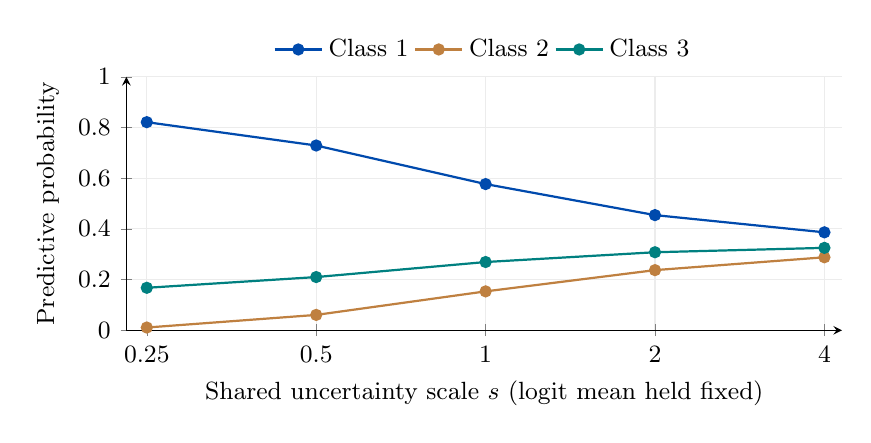
\begin{tikzpicture}
\begin{axis}[width=.88\textwidth,height=4.8cm,
xmode=log,log basis x=2, xmin=.23,xmax=4.3,ymin=0,ymax=1,
xtick={.25,.5,1,2,4},xticklabels={0.25,0.5,1,2,4},
xlabel={Shared uncertainty scale $s$ (logit mean held fixed)},
ylabel={Predictive probability},grid=major,grid style={gray!15},
axis lines=left, tick label style={font=\small},label style={font=\small},
legend style={draw=none,at={(.5,1.02)},anchor=south,legend columns=3,font=\small}]
\addplot[thick,mark=*,mark size=1.8pt,revisionblue] coordinates {(0.25,0.821321935) (0.5,0.729192611) (1.0,0.577012102) (2.0,0.454552028) (4.0,0.386587378)};\addlegendentry{Class 1}
\addplot[thick,mark=*,mark size=1.8pt,brown] coordinates {(0.25,0.010943193) (0.5,0.060729307) (1.0,0.153583550) (2.0,0.237426353) (4.0,0.288134325)};\addlegendentry{Class 2}
\addplot[thick,mark=*,mark size=1.8pt,teal] coordinates {(0.25,0.167734872) (0.5,0.210078082) (1.0,0.269404347) (2.0,0.308021619) (4.0,0.325278297)};\addlegendentry{Class 3}
\end{axis}\end{tikzpicture}
% END SCALE_PLOT
\caption{The shared deviation scale changes predictive probabilities while the logit mean is held fixed. Each curve uses the variance-mixture Laplace-Remax equations. This is a constructed state, not a trained-network calibration experiment.}
\label{F:scale}
\end{figure}
The batch-reference calibration labels are generated at $s=1.8$ for this fixed input; fitting \eqref{E:calobjective} reduces population cross-entropy. This verifies a batch calibration reference, not the sequential recursion or trained-network calibration. The script also checks the Gaussian channel, the identity update for $K=1$, and invariance when every logit mean is zero. Extreme CDF saturation, very rare classes, and large $K$ require further numerical checks.

\paragraph{Auxiliary-channel check.}
For the same three-class state, a prior $L\sim\Normal(0.1,0.2^2)$ and observed class $C=2$ give
\begin{equation}
\lambda^+=0.132152,\quad q^+_{\rm event}=0.0397933,\quad
q^+_{\rm full}=0.0396814,\quad q^+_{\rm tilt}=0.0385930.
\end{equation}
The script \texttt{verification/check\_auxiliary\_channel.py} verifies the common posterior-mean identity, both expected-variance identities, and the full categorical sum formula. Refining the scale quadrature from 20 to 32 nodes changes these moments by less than $3\times10^{-16}$ in this setting. These are one-step checks; they do not establish the repeated-pass calibration performance of the auxiliary recursion.

\appendix
\section{Optional direct categorical training}\label{S:training}
This extension changes the training likelihood; it is optional and is not part of the original two-channel calibration design. During training fix $L=0$. Write $\bm X=\bm Z+\bm V$ and specify the observed label by
\begin{equation}
\boxed{C\given\bm Z,\bm U,\bm\xi\sim\operatorname{Categorical}(\Remax(\bm Z+\sqrt{\bm h(\bm U)}\odot\bm\xi)).}
\label{E:catmodel}
\end{equation}
The square root and product are componentwise. A label is observed once; neither $\bm A$ nor $\bm V$ is observed. The likelihood after integrating $\bm\xi$ is well-defined and includes aleatoric noise before normalization. This is a categorical extension of the TAGI-V architecture, not the Gaussian regression likelihood used in the original formulation.

For the current Gaussian prior summary, a label $C=c$ gives the tilted distribution
\begin{equation}
\widetilde q(\bm z,\bm u,\bm\xi\given c)
=\frac{A_c\,q(\bm z,\bm u)\prod_j\varphi(\xi_j)}{m_c(0)}.
\label{E:tilt}
\end{equation}
For either output state $T_j\in\{Z_j,U_j\}$, the posterior moments are
\begin{equation}
\boxed{
\mu_{T_j}^+=\frac{\E[T_jA_c]}{m_c(0)},\qquad
(\sigma_{T_j}^2)^+=\frac{\E[T_j^2A_c]}{m_c(0)}-(\mu_{T_j}^+)^2.
}\label{E:tiltedmoments}
\end{equation}
These are exact tilted marginal moments under the working prior. The updated marginals are then projected to a factorized Gaussian; repeated projections and TAGI backward inference remain approximations. A posterior variance may increase after an unexpected class, so a variance update should not be forced to be negative merely because a Kalman observation update would decrease it.

\subsection{Tractable marked kernels}
All kernels in this subsection use $L=0$. For $r\in\{1,2\}$, define
\begin{equation}
T_{j,r}(t)=\E[T_j^r e^{-tM_j}],\quad
D_{j,r}^{(T)}(t)=\E[T_j^rM_j e^{-tM_j}],\quad
n_{j,r}^{(T)}=\E[T_j^r\ind_{X_j\le0}].
\label{E:marked}
\end{equation}
Here $T_{j,r}$ is a marked kernel, not the latent variable $T_j$ itself. Independence between classes and the same Laplace identity yield
\begin{equation}
\E[T_j^rA_c]=
\begin{cases}
\displaystyle\int_0^\infty D_{c,r}^{(T)}(t)\prod_{k\ne c}L_k(t)\dd t
+\dfrac{n_{c,r}^{(T)}}K\prod_{k\ne c}\pi_{0,k},&j=c,\\[.9em]
\displaystyle\int_0^\infty D_c(t)T_{j,r}(t)\prod_{k\notin\{c,j\}}L_k(t)\dd t
+\dfrac{n_{j,r}^{(T)}}K\prod_{k\ne j}\pi_{0,k},&j\ne c.
\end{cases}
\label{E:markedtilt}
\end{equation}
Appendix~\ref{A:marked} gives explicit formulas requiring only scalar integration over $U_j$. In particular, factors $U_j$ and $U_j^2$ in these kernels allow the label to update the variance head even though its covariance with the raw zero-mean error is zero. Diagonal posterior moments for both heads cost $O(QJK)$ for one observed class; a dense class Jacobian is unnecessary.


Once the two-head posterior moments are obtained, use the common RTS equations in \S\ref{S:gaussian}. This optional route supplies a coherent categorical training likelihood; the default Gaussian-channel route instead preserves the training/calibration separation of the intended source.

\section{Explicit kernels for categorical updates}\label{A:marked}
This appendix provides the missing computations in \eqref{E:markedtilt}. During training, $s=1$. Conditional on $U=u$, set $h=h(u)$, $d^2=e+h$, and $m=\mu$. Then $(Z,X)\given u$ is jointly Gaussian, with
\begin{equation}
\E[Z\given X,u]=a+bX,\qquad
b=\frac{e}{e+h},\quad a=\mu(1-b),\qquad
\Var(Z\given X,u)=c=\frac{eh}{e+h}.
\label{E:ZXregress}
\end{equation}
In this appendix $a,b,c$ are local regression coefficients, unrelated to the CDF arguments or the class label. Define the negative-side moments
\begin{align}
p_0&=\Phi(-m/d),\\
N&=mp_0-d\varphi(m/d),\\
R&=(m^2+d^2)p_0-md\varphi(m/d).
\end{align}
In addition to $\mathcal L,\mathcal D,\mathcal F$ in \eqref{E:kernels}, use
\begin{align}
\mathcal G(t)&:=\E[M^3e^{-tM}]\nonumber\\
&=c_0(t)\left[(b_0(t)^3+3b_0(t)d^2)\Phi(\beta(t))
+d(b_0(t)^2+2d^2)\varphi(\beta(t))\right],\\
b_0(t)&=m-d^2t,\qquad c_0(t)=\exp(-mt+d^2t^2/2).
\end{align}
Since $X=M$ on $X>0$, $\E[Xe^{-tM}]=N+\mathcal D$ and $\E[X^2e^{-tM}]=R+\mathcal F$. Consequently the conditional marked kernels for $Z$ are
\begin{align}
\E[Ze^{-tM}\given u]&=a\mathcal L+b(N+\mathcal D),\\
\E[Z^2e^{-tM}\given u]&=(c+a^2)\mathcal L+2ab(N+\mathcal D)+b^2(R+\mathcal F),\\
\E[ZMe^{-tM}\given u]&=a\mathcal D+b\mathcal F,\\
\E[Z^2Me^{-tM}\given u]&=(c+a^2)\mathcal D+2ab\mathcal F+b^2\mathcal G,\\
\E[Z\ind_{X\le0}\given u]&=ap_0+bN,\\
\E[Z^2\ind_{X\le0}\given u]&=(c+a^2)p_0+2abN+b^2R.
\label{E:zmarks}
\end{align}
For the variance latent state, simply use
\begin{equation}
\E[U^re^{-tM}\given u]=u^r\mathcal L,\quad
\E[U^rMe^{-tM}\given u]=u^r\mathcal D,\quad
\E[U^r\ind_{X\le0}\given u]=u^rp_0.
\end{equation}
Average each expression over $U\sim\Normal(\nu,r)$ to obtain \eqref{E:marked}. The desired input-output cross-covariance is also available from the $r=1$ numerator:
\begin{equation}
\Cov(T_j,A_c)=\E[T_jA_c]-\mu_{T_j}m_c(0).
\end{equation}
No missing covariance formula needs to be imported from a lognormal approximation.

\section{Within-class head correlation and numerical details}\label{A:correlated}
\subsection{Retaining a correlated pair}
Independence between classes is the key Laplace factorization assumption. It is possible to retain a $2\times2$ block for each $(Z_i,U_i)$ without changing the scalar nature of \eqref{E:mixturekernels}. Let $c_i=\Cov(Z_i,U_i)$ and $r_i>0$. Then
\begin{equation}
Z_i\given U_i=u\sim\Normal\!\left(\mu_i+\frac{c_i}{r_i}(u-\nu_i),\ e_i-\frac{c_i^2}{r_i}\right).
\end{equation}
Use
\begin{equation}
m_i(u,l)=\mu_i+e^l\frac{c_i}{r_i}(u-\nu_i),\qquad
d_i^2(u,l)=e^{2l}\left[e_i-\frac{c_i^2}{r_i}+h(u)\right]
\end{equation}
in the Gaussian kernels. In Appendix~\ref{A:marked}, also replace $\mu$ by $\E[Z_i\given u]$ and $e$ by $\Var(Z_i\given u)$ in the conditional regression coefficients. The unconditional variance is still $e^{2l}(e_i+h_i)$. Cross-head posterior moments follow by multiplying the $Z$ marked kernels by $u$ and using the same tilt. Cross-class correlations require further conditioning or a different integration scheme and are not handled by the independent product formulas.

\subsection{Stable evaluation and degeneracies}
For $\beta<0$, the positive part of $\mathcal L$ can be evaluated using
\begin{equation}
c(t)\Phi(\beta(t))=\tfrac12e^{-\alpha^2/2}\operatorname{erfcx}(-\beta(t)/\sqrt2).
\end{equation}
The higher kernels require stable truncated-normal moments or asymptotic expansions; merely stabilizing the exponential does not remove cancellation in $\mathcal D,\mathcal F,\mathcal G$. For example, write their positive moments as
\begin{equation}
\E[M^n e^{-tM}]=d^n\varphi(\alpha)\int_0^\infty y^n e^{-y^2/2+\beta y}\dd y,
\end{equation}
and evaluate the integral directly with stable special functions or tail expansions. The verification script uses a parabolic-cylinder representation and a negative-tail expansion for this integral. Its test range does not cover every extreme positive-tail regime.

A convenient Laplace integration map is $t=y/[a(1-y)]$ for $y\in(0,1)$, where $a>0$ is a typical positive rectified-sum scale, with $\dd t=\dd y/[a(1-y)^2]$. For variance heads, normalized Gauss--Hermite nodes $x_j,w_j$ give $\E[f(U)]\approx\sum_jw_jf(\nu+\sqrt r\,x_j)$. Increase both orders until predictive probabilities \emph{and training second moments} converge. Check scale integration separately and enlarge its domain until tail mass is negligible. Use log likelihoods and stable normalization for surprising labels.

Preserve the uniform all-zero policy in prediction, posterior moments, and verification. Handle deterministic $r_i=0$ by evaluating at $U_i=\nu_i$. The positive variance floor keeps the conditional predictive $d_i$ nonzero for finite $l$; if a zero-floor variant is implemented, handle degenerate Gaussian logits explicitly. Any numerical covariance repair should be restricted to verified roundoff errors; a large violation of \eqref{E:simplexchecks} indicates insufficient accuracy or inconsistent moments.

\section{Source mapping and status of the contributions}\label{A:sources}
The template and calibration design are taken from the user-supplied \nolinkurl{HSM_calibration_Goulet_Nguyen_Florensa.original.tex}. Its effective page geometry, line spacing, two-line Polytechnique header, timestamp footer, and direct start with \emph{Context} are reproduced; the header height is set explicitly to accommodate its two lines. The course title is adapted to this Remax note. Its Gaussian auxiliary observation channel, observed-event encoding, expected Bernoulli variance, scalar Gaussian update, and epoch-wise tracking option are the principal methodological starting points.

The original tree and its node gains are replaced by a multiclass Remax transform and one common deviation scale. Gaussian-CDF moments remain exact for Gaussian inputs. In the original gain-product construction, however, differentiating a GMA approximation to a predictive mean does not turn the resulting covariance into an exact covariance of the non-Gaussian product. Here scale moments and cross-covariances are computed by conditional integration, with approximation labels kept explicit. The positivity parameterization and the interpretation of repeated-epoch resets are stated separately from the source's practical rules.

The supplied \nolinkurl{ATRTCT_v2.pdf}, \S4.2 and Appendix A.2, supplies the MM-Remax baseline. The supplied \nolinkurl{laplace_remax_theory.pdf}, \S\S3--7 and 13, supplies Gaussian Laplace kernels, the uniform all-zero convention, and the optional categorical-tilt principle. The variance-mixture kernels, centered shared scale, and application of the original auxiliary channel to their moments are proposed here. The main training/calibration separation follows the intended original note; the optional categorical network-training extension is not attributed to it.

Numerical checks concern these equations and constructed calibration examples. The source note's reported HSM experiments are not reused as evidence for the proposed Remax formulation.

\clearpage
\begin{thebibliography}{9}
\bibitem{goulet2021}
J.-A. Goulet, L.-H. Nguyen, and S. Amiri.
\newblock Tractable approximate Gaussian inference for Bayesian neural networks.
\newblock \emph{Journal of Machine Learning Research}, 22(251):1--23, 2021.
\newblock \url{https://jmlr.org/papers/v22/20-1009.html}.
\bibitem{dekav}
B. Deka, L.-H. Nguyen, and J.-A. Goulet.
\newblock Analytically tractable heteroscedastic uncertainty quantification in Bayesian neural networks for regression tasks.
\newblock \emph{Neurocomputing}, article 127183; author preprint dated January 12, 2024.
\newblock \url{https://profs.polymtl.ca/jagoulet/Site/Papers/Deka_TAGIV_2024_preprint.pdf}.
\bibitem{agvi}
B. Deka and J.-A. Goulet.
\newblock Approximate Gaussian variance inference for state-space models.
\newblock \emph{International Journal of Adaptive Control and Signal Processing}, 37(11):2934--2962, 2023.
\newblock \url{https://doi.org/10.1002/acs.3667}.
\bibitem{mm}
\emph{Analytically Tractable Real-to-Categorical Transformations for Bayesian Neural Networks}.
\newblock User-supplied manuscript, \nolinkurl{ATRTCT_v2.pdf}, accessed September 10, 2026.
\bibitem{laplace}
\emph{Laplace-Remax: Moment Propagation for Normalized Rectified Gaussian Classifiers}.
\newblock User-supplied TAGI note dated June 17, 2026, \nolinkurl{laplace_remax_theory.pdf}.
\bibitem{hsm}
J.-A. Goulet, L.-H. Nguyen, and M. Florensa-Montilla.
\newblock \emph{Hierarchical Softmax Calibration}.
\newblock User-supplied original \LaTeX{} note and template, \nolinkurl{HSM_calibration_Goulet_Nguyen_Florensa.original.tex}, accessed September 10, 2026.
\end{thebibliography}
\end{document}
